\documentclass{article}
\usepackage{graphicx, float} % Required for inserting images
\usepackage[letterpaper, margin=1in]{geometry}
\usepackage{amsfonts, amsmath, hyperref, leftindex, listings, multirow, physics, placeins, thmtools}

\DeclareMathOperator{\Grad}{grad}
\DeclareMathOperator{\Div}{div}
\DeclareMathOperator{\Curl}{curl}

\newcommand{\vddot}{\boldsymbol{:}}

\title{EpiPINN: Neural Network for Parameter Estimation of Epidemic Model}
\author{Ashton Cole}
\date{\today}

\begin{document}
	\maketitle
	
	\section{Introduction}
	\label{section:Introduction}
	
	In this project, we attempted to replicate the work of \cite{zinihi_identifying_2025}, using a physics-informed neural network (PINN) to learn epidemic data and estimate the parameters for a fractional-order SEIRD model. We had some difficulties in implementing parts of the paper, and the PINN did not learn SEIRD parameters accurately. In conclusion, more development is necessary for PINNs to be a reliable choice for epidemic modeling.
	
	\subsection{Caputo Fractional Calculus}
	\label{subsection:Caputo_Fractional_Calculus}
	
	The Caputo fractional derivative and integral are a means of extending derivatives and integrals past integer orders. The Caputo integral and derivative for $\alpha \in (0, 1]$  are defined using convolutions.
	
	\begin{align}
		^{\mathcal{C}}\mathcal{I}_{t}^{\alpha} [f] (t) &= \frac{1}{\Gamma(\alpha)} \int_{0}^{t} (t - \tau)^{\alpha - 1} f(\tau) \dd{\tau} \\
		^{\mathcal{C}}\mathcal{D}_{t}^{\alpha} [f] (t) &= \frac{1}{\Gamma(1- \alpha)} \int_{0}^{t} (t - \tau)^{-\alpha} f'(\tau) \dd{\tau}
	\end{align}
	
	Because the fractional derivative requires integration from an initial time, it is dependent on the function globally, as opposed to being an instantaneous rate of change. This dependence is referred to as memory effects.
		
	\subsection{SEIRD Model}
	\label{subsection:SEIRD_Model}
	
	The SEIRD Model is an extension of the SIR compartmental model, used to model pandemic progression. The population is divided into five compartments: susceptible, exposed, infected, recovered, and dead. Changes the compartments are defined by the following system of ordinary differential equations.
	
	\begin{align}
		\dv{S}{t} &= -\beta \frac{S I}{N - D} \\
		\dv{E}{t} &= \beta \frac{S I}{N - D} - \sigma E \\
		\dv{I}{t} &= \sigma E - (\gamma + \mu) I \\
		\dv{R}{t} &= \gamma I \\
		\dv{D}{t} &= \mu I
	\end{align}
	
	Susceptible people are exposed at an infection rate $\beta$, exposed people become infected at an incubation rate $\sigma$, and infected people either recover at a recovery rate $\gamma$ or die at a mortality rate $\mu$. Importantly, the whole population $N = S + E + I + R + D$ is conserved.
	
	The paper replaces these first-order derivatives with the Caputo fractional ones, all of some order $\alpha$. In the ODE model, the rate of change of each compartment at a given time is dependent only on the state of that population at the same instant. Fractional differential equations (FDEs), however, make present dynamics dependent on the past, and have been shown to better fit epidemic data. The modified system, with compartments normalized by total population $N$, are shown below.
	
	\begin{align}
		^{\mathcal{C}}\mathcal{D}_{t}^{\alpha} [s] &= -\beta \frac{s i}{1 - d} \\
		^{\mathcal{C}}\mathcal{D}_{t}^{\alpha} [e] &= \beta \frac{s i}{1 - d} - \sigma e \\
		^{\mathcal{C}}\mathcal{D}_{t}^{\alpha} [i] &= \sigma e - (\gamma + \mu) i \\
		^{\mathcal{C}}\mathcal{D}_{t}^{\alpha} [r] &= \gamma i \\
		^{\mathcal{C}}\mathcal{D}_{t}^{\alpha} [d] &= \mu i
	\end{align}
	
	A potential flaw of fractional derivatives, however, is that they introduce unintuitive and nonphysical behavior. Although fractional derivatives will still conserve the total, they cause undesired movement between compartments. For example, notice how in Figure \ref{figure:alpha_effect}, after about 200 days, the number of susceptible people $s$ increases, while recovered people $r$ decreases. In the ODE case, this would be impossible, as their derivatives are strictly negative and positive, respectively. For a fractional derivative, however, a positive value does not always correspond to an increase, or vice-versa. Perhaps memory effects are useful in the initial stages of an epidemic, but clearly fractional derivatives fail at predicting long-term equilibrium. This behavior was not considered in the paper.
	
	\begin{figure}
		\centering
		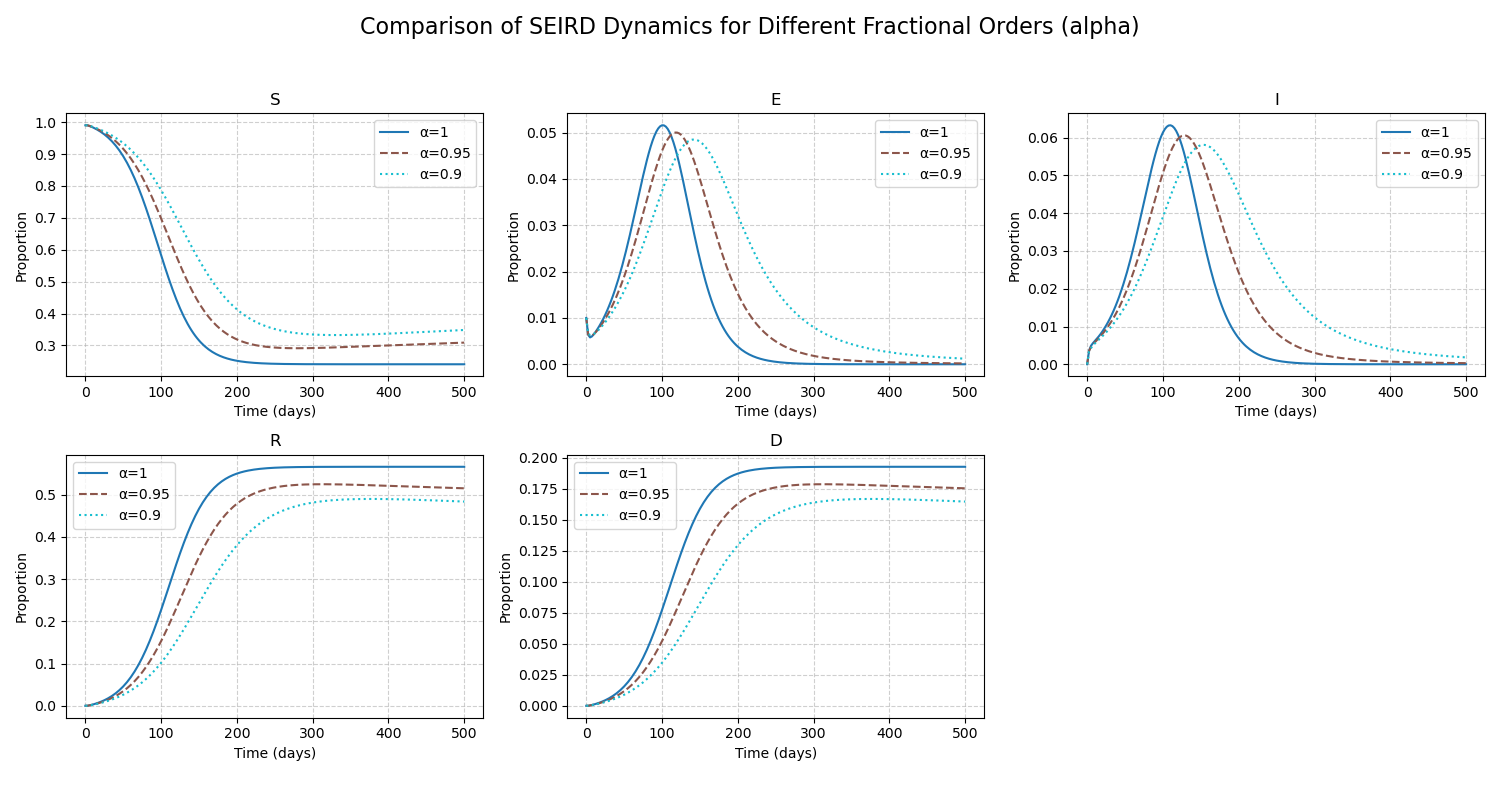
\includegraphics[width=\linewidth]{images/alpha_effect.png}
		\caption{Normalized SEIRD dynamics for different fractional orders $\alpha$.}
		\label{figure:alpha_effect}
	\end{figure}
	
	\section{Methodology}
	\label{section:Methodology}
	
	In this section, we discuss our implementation of the work in the paper. We successfully implemented fractional calculus, the PINN, and training as described. However, we were not able to find the referenced compartmental time series, instead opting to generate our own data.
	
	\subsection{Implementation of Caputo Fractional Calculus}
	\label{subsection:Implementation_of_Caputo_Fractional_Calculus}
	
	The Caputo fractional derivative was implemented for discrete time series of fixed step. The L1 scheme is used, meaning that the continuous definition is made discrete by approximating the function as piecewise linear between points. The following equation results, and is made very efficient by rewriting as a Toeplitz matrix multiplication.
	
	\begin{align}
		f'_{0} &= 0 \\
		f'_{k + 1} &= \frac{1}{\Gamma(2 - \alpha)} \sum_{j = 0}^{k} \frac{f(t_{j + 1}) - f(t_{j})}{t_{j + 1} - t_{j}} \left( (t_{k + 1} - t_{j})^{1 - \alpha} - (t_{k + 1} - t_{j + 1})^{1 - \alpha} \right) \\
		&= \frac{(\Delta t)^{-\alpha}}{\Gamma(2 - \alpha)} \sum_{j = 0}^{k} \left( f(t_{j + 1}) - f(t_{j}) \right) \left( (k + 1 - j)^{1 - \alpha} - (k - j)^{1 - \alpha} \right) \\
		&= \frac{(\Delta t)^{-\alpha}}{\Gamma(2 - \alpha)} \sum_{j = 0}^{k} \Delta f_{j} w_{k - j} \\
		\Delta f_{j} &= f(t_{j + 1}) - f(t_{j}) \\
		w_{k - j} &= (k + 1 - j)^{1 - \alpha} - (k - j)^{1 - \alpha} \\
		\bmqty{
			f'_{1} \\
			f'_{2} \\
			f'_{3} \\
			\vdots
		} &= \bmqty{
			w_{0} &  &  &   \\
			w_{1} & w_{0} &  &  \\
			w_{2} & w_{1} & w_{0} &  \\
			\vdots & \vdots & \vdots & \ddots
		} \bmqty{
			\Delta f_{1} \\
			\Delta f_{2} \\
			\Delta f_{3} \\
			\vdots
		}
	\end{align}
	
	The Caputo-Euler method for a FDE $^{\mathcal{C}}\mathcal{D}_{t}^{\alpha} [\vb{y}] = f(t, \vb{y})$ is implemented with a similar form, but must be computed in a loop.
	
	\begin{align}
		\vb{y}_{k + 1} &= \vb{y}_{0} + \frac{(\Delta t)^{\alpha}}{\Gamma(\alpha + 1)} \sum_{j = 0}^{k} f(t_{j}, \vb{y}_{j}) \left( (k + 1 - j)^{1 - \alpha} - (k - j)^{1 - \alpha} \right) \\
		&= \vb{y}_{0} + \frac{(\Delta t)^{\alpha}}{\Gamma(\alpha + 1)} \sum_{j = 0}^{k} \vb{f}_{j} w_{k - j} \\
		\vb{f}_{j} &= f(t_{j}, \vb{y}_{j}) \\
		w_{k - j} &= (k + 1 - j)^{1 - \alpha} - (k - j)^{1 - \alpha}
	\end{align}
	
	\subsection{Implementation of Neural Network}
	\label{subsection:Implementation_of_Neural_Network}
	
	We implemented a PINN in PyTorch based on the structure described in the paper. The network models the state as a function of time, $(s, e, i, r, d) = NN(t)$. It has one input dimension and five output dimensions. Perceptron dimenions were not specified, so after some experimentation, a sequential neural network with three layers of 64 perceptrons was assumed. Tanh activation functions are used between layers, while a softmax function is applied to the output layer to force normalized population conservation. Fractional order and FDE coefficients and $\alpha, \beta, \sigma, \gamma, \mu$ are included as trainable parameters, but are not stored directly. To ensure positivity for the disease rates, raw scores are stored internally, and a softplus function is applied whenever they are used. Meanwhile, for $\alpha$, the range is restricted to $(\alpha_{\mathrm{min}}, 1)$ by a scaled sigmoid function.
		
	\subsection{Training Process}
	\label{subsection:Training_Process}
	
	Training takes place in two stages, outlined in table \ref{table:stages}. The first stage fits the data, and the second learns the FDE. First, weights are initialized using uniform Xavier initialization. The following losses are used for training.
	
	\begin{align}
		\mathcal{L}_{\mathrm{data}} &= \frac{1}{N} \sum_{n = 1}^{N} \norm{(s(t_{n}), e(t_{n}), i(t_{n}), r(t_{n}), d(t_{n})) - NN(t_{n})}_{2}^{2} \\
		\mathcal{L}_{\mathrm{IC}} &= \norm{(s_{0}, e_{0}, i_{0}, r_{0}, d_{0}) - NN(t_{0})}_{2}^{2} \\
		\mathcal{L}_{\mathrm{phys}} &= \frac{1}{M} \sum_{m = 1}^{M} \norm{^{\mathcal{C}}\mathcal{D}_{t}^{\alpha} [NN](\hat{t}_{n}) - f(t_{n}, NN(\hat{t}_{m}))}_{2}^{2}
	\end{align}
	
	Data loss is the MSE of predictions against data. IC loss is the MSE of the initial condition. Physics loss is the square norm of the FDE residual computed at collocation points $\hat{t}_{m}$, where the FDE is $^{\mathcal{C}}\mathcal{D}_{t}^{\alpha} [(s, e, i, r, d)] = f(t, (s, e, i, r, d))$. Unlike in the paper, conservation loss is not implemented directly. but, instead enforced on the output with softmax.
	
	Both training stages are relatively standard. They just minimize different objectives and train different parameters. Early stopping is implemented in both with a patience counter. If loss does not improve after a certain number of epochs, training stops. The second stage uses the L-BFGS optimizer, because it is shown to work well for parameter estimation in the literature.
		
	\begin{table}
		\centering
		\caption{Configuration for each training stage.}
		\begin{tabular}{c|ccc}
			 & Parameters Trained & Loss Function & Optimizer \\
			\hline
			Stage 1 & $\Theta$ & $\mathcal{L}_{\mathrm{data}} + \mathcal{L}_{\mathrm{IC}}$ & Adam \\
			Stage 2 & $\Theta, \alpha, \beta, \gamma, \mu$ & $\mathcal{L}_{\mathrm{data}} + \mathcal{L}_{\mathrm{IC}} + 10,000 \mathcal{L}_{\mathrm{phys}}$ & L-BFGS
		\end{tabular}
		\label{table:stages}
	\end{table}
	
	\section{Results and Discussion}
	\label{section:Results_and_Discussion}
	
	Two experiments were conducted to evaluate the PINN. In experiment 1, it was trained on FDE ground truth data. Stage 1 ran for 5000 epochs using a learning rate of 1e-3 and weight decay 1e-5. Stage 2 ran for 5,000 epochs using a learning rate of 1e-5. Physics loss was weighted by a factor of 1e4 to emphasize FDE residual convergence. After initial training, the model fit the FDE solution quite well, but after stage 2, the neural network had a worse fit. Unlike the paper, we also studied parameter convergence across epochs. Epidemiological parameters seemed to converge quite quickly, but did so to incorrect values. Clearly, this reduced the physics loss computation, but lead to a worse overall.
		
	For experiment 2, a similar setup was used, but noise was added to the data. Parameters were additionally randomized to a similar range. Again, stage 2 of training led to a worse data fit, and eoidemiological parameters converged to inaccurate values.
	
	\begin{table}
		\centering
		\caption{Epidemiological parameters for experiment 1.}
		\begin{tabular}{c|ccccc}
			 & $\alpha$ & $\beta$ & $\gamma$ & $\sigma$ & $\mu$ \\
			 \hline
			 Exact & 0.994 & 0.166 & 0.117 & 0.077 & 0.02 \\
			 \hline
			 Initial Guess & 0.96 & 0.26 & 0.14 & 0.053 & 0.006 \\
			 Estimate & 0.962 & 0.151 & 0.0789 & 0.116 & 0.00662
		\end{tabular}
		\label{table:experiment1}
	\end{table}
	
	\begin{figure}
		\centering
		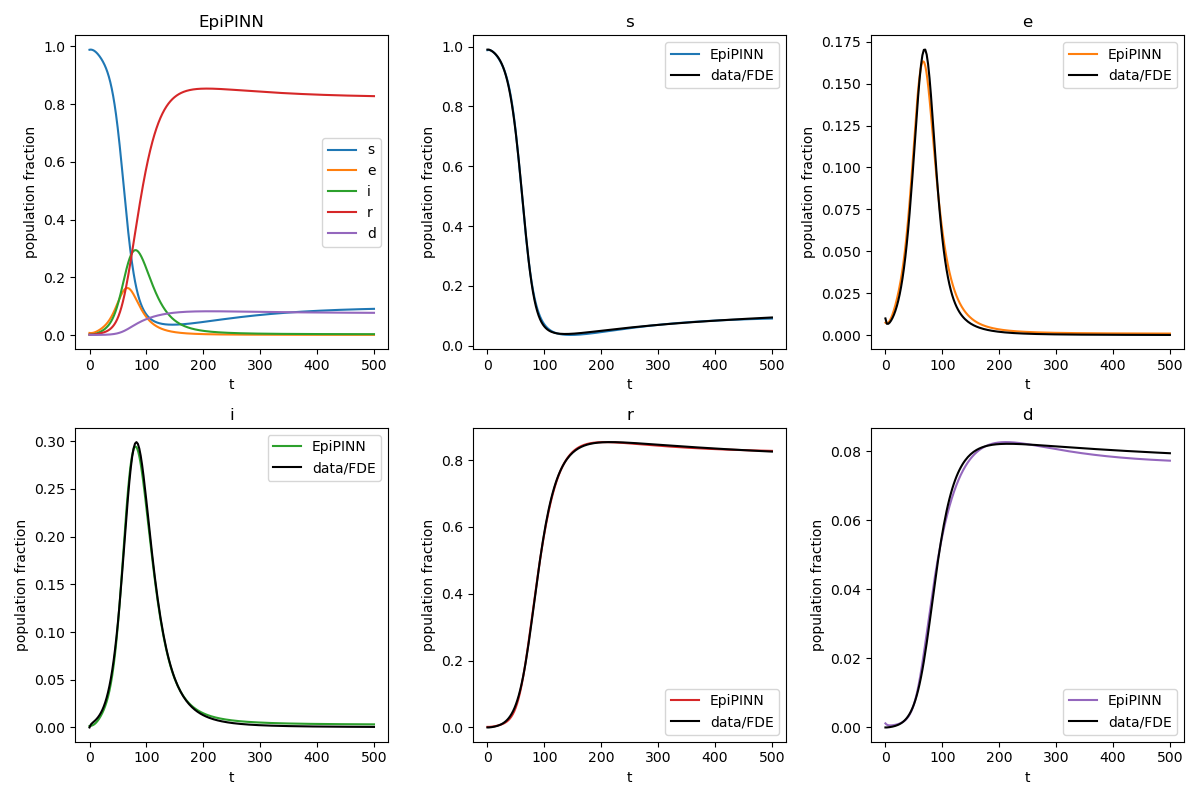
\includegraphics[width=0.49\linewidth]{images/experiment1_stage1.png}
		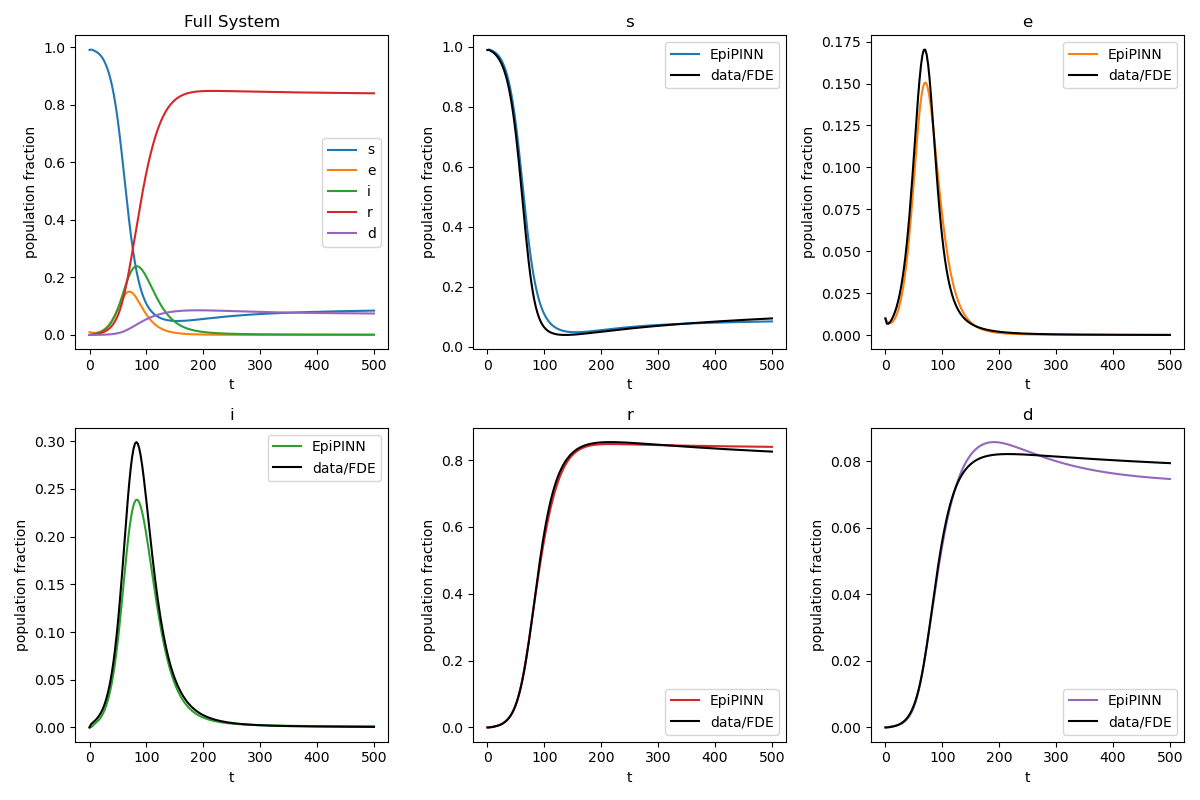
\includegraphics[width=0.49\linewidth]{images/experiment1_stage2.png}
		\caption{Experiment 1 model outputs after stages 1 and 2.}
		\label{figure:experiment1_outputs}
	\end{figure}
	
	\begin{figure}
	\centering
	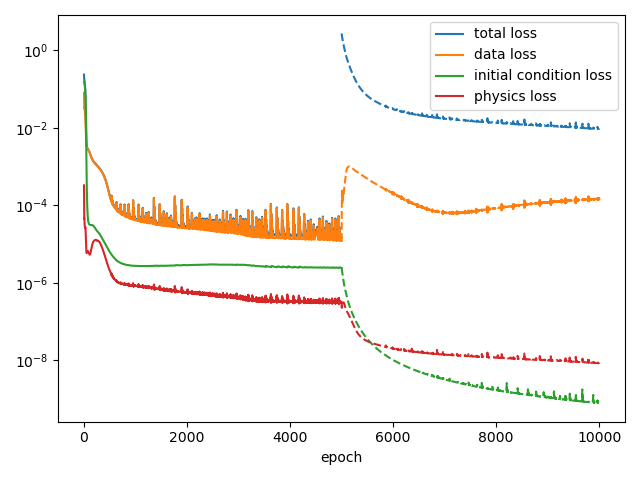
\includegraphics[width=0.44\linewidth]{images/experiment1_losses.png}
	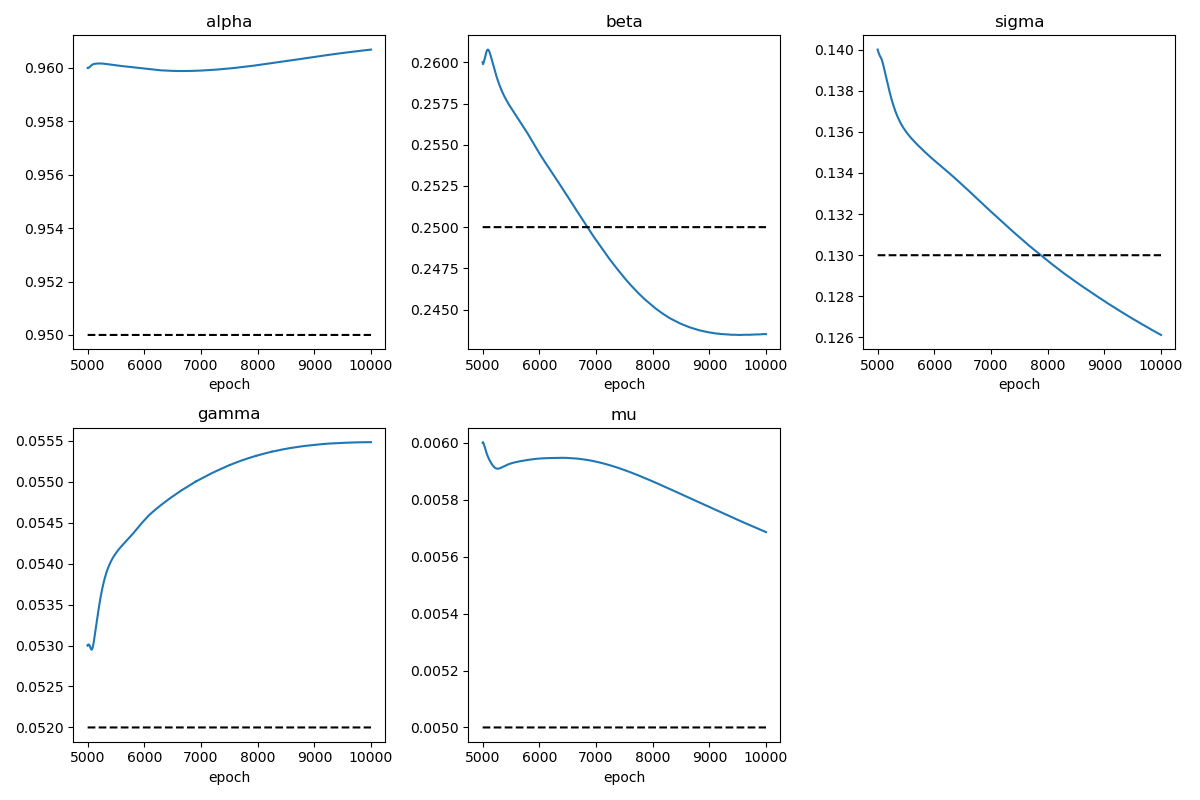
\includegraphics[width=0.49\linewidth]{images/experiment1_parameters.png}
	\caption{Experiment 1 loss and parameter convergence.}
	\label{figure:experiment1_losses}
	\end{figure}
	
	\begin{table}
		\centering
		\caption{Epidemiological parameters for experiment 2.}
		\begin{tabular}{c|ccccc}
			& $\alpha$ & $\beta$ & $\gamma$ & $\sigma$ & $\mu$ \\
			\hline
			Exact & 0.95 & 0.25 & 0.13 & 0.052 & 0.005 \\
			\hline
			Initial Guess & 0.96 & 0.26 & 0.14 & 0.053 & 0.006 \\
			Estimate & 0.959 & 0.246 & 0.0534 & 0.121 & 0.00587
		\end{tabular}
		\label{table:params2}
	\end{table}
	
	\begin{figure}
		\centering
		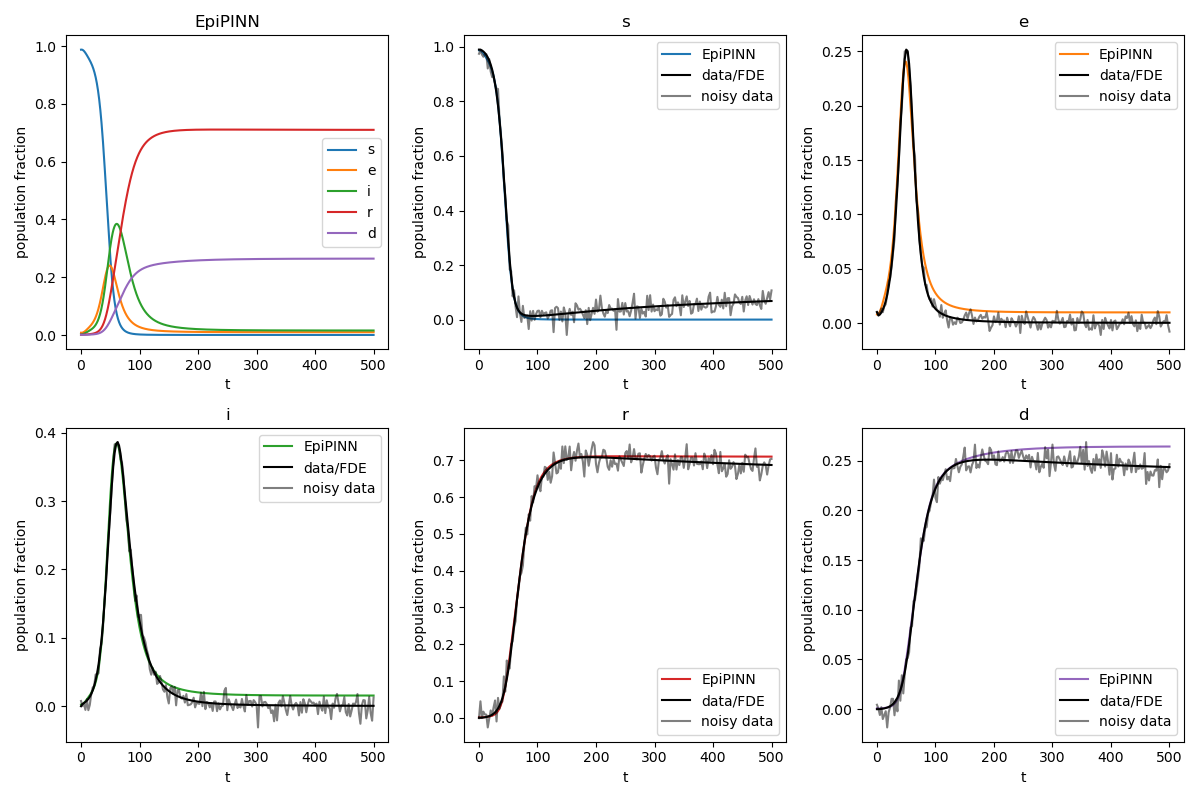
\includegraphics[width=0.49\linewidth]{images/experiment2_stage1.png}
		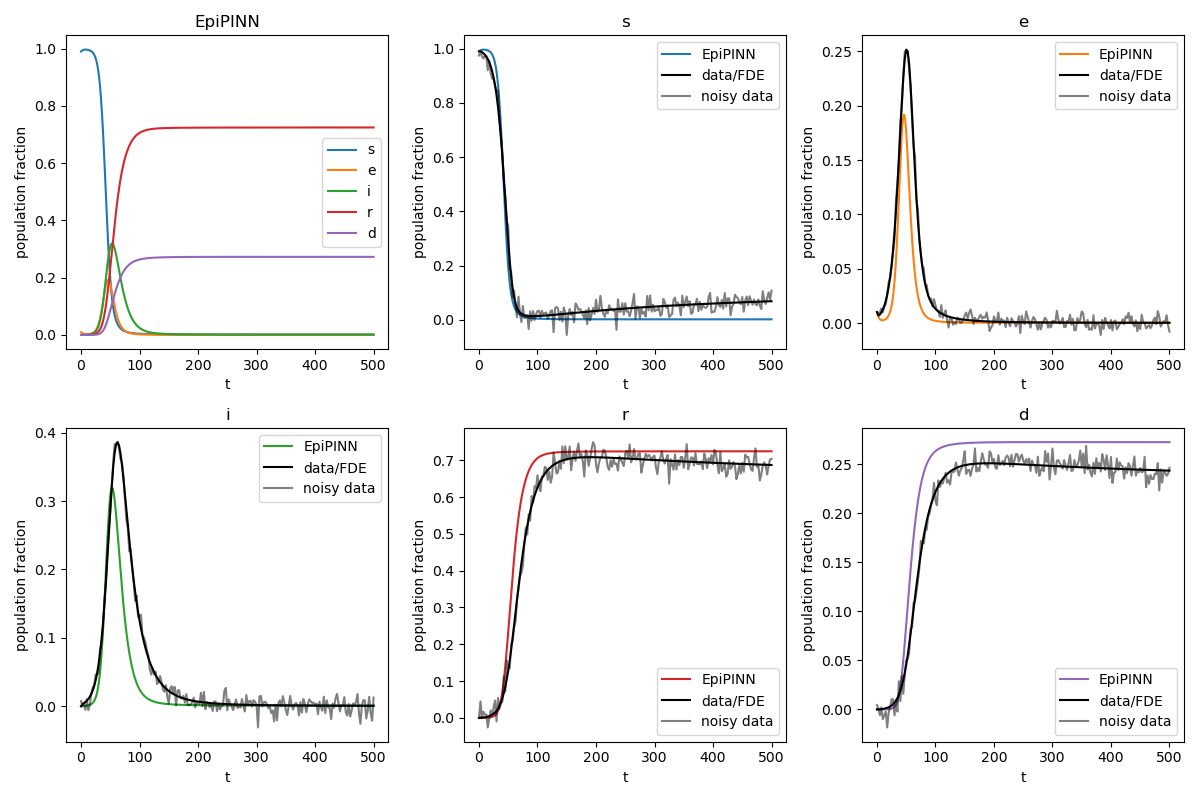
\includegraphics[width=0.49\linewidth]{images/experiment2_stage2.png}
		\caption{Experiment 1 model outputs after stages 1 and 2.}
		\label{figure:experiment2_outputs}
	\end{figure}
	
	\begin{figure}
		\centering
		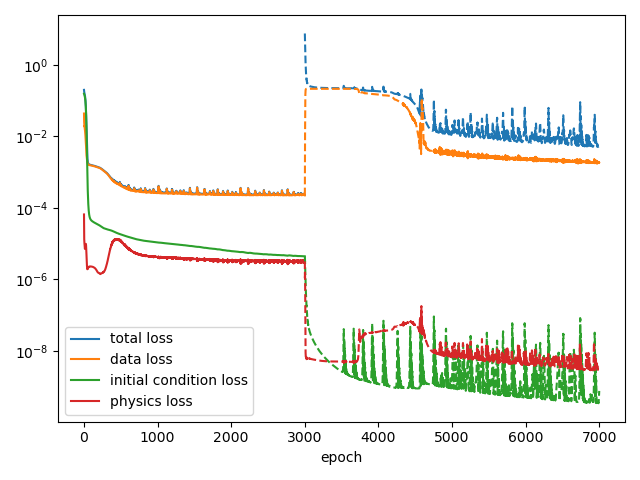
\includegraphics[width=0.44\linewidth]{images/experiment2_losses.png}
		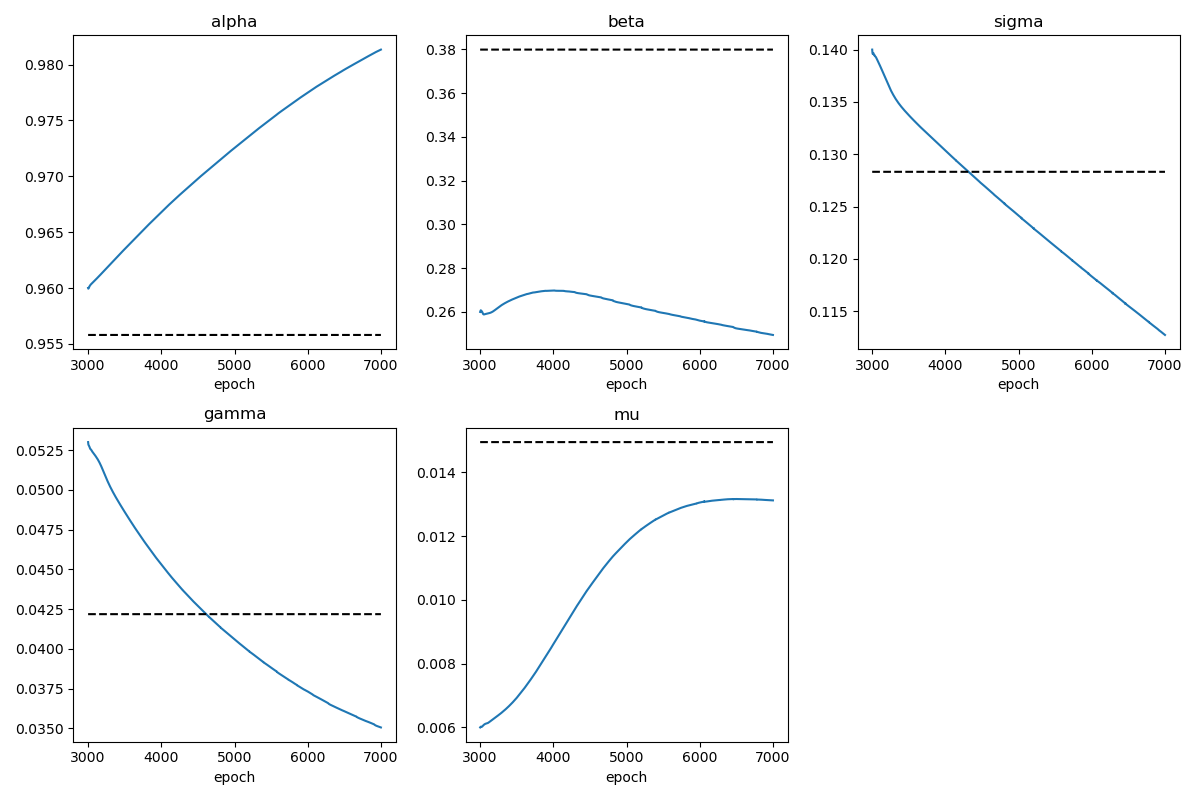
\includegraphics[width=0.49\linewidth]{images/experiment2_parameters.png}
		\caption{Experiment 1 loss and parameter convergence.}
		\label{figure:experiment2_losses}
	\end{figure}
	
	\section{Conclusions}
	\label{section:Conclusions}
	
	In conclusion, while the network seemed to converge with precision, it did so to unacceptably inaccurate values, particularly for FDE-generated data. It is possible that too many degrees of freedom were added to the physics FDE. With split objectives of minimizing data and FDE residual loss, the model seems to prefer fitting the network to a new FDE as opposed to recovering the original FDE. We also have questions about the paper's accuracy. From the table they provided, it is clear that their PINN, like our own, generally predicts values in the neighborhood of the correct ones, but they do not provide initial guesses and convergence plots.
	
	We successfully implemented the model described in the paper. However, imrpoving parameter convergence is a major concern to address before such a model could be used to reliably model epidemics.
	
	\bibliographystyle{plain}
	\bibliography{refs}
\end{document}